\documentclass[../../statistical_learning_notes.tex]{subfiles}
\begin{document}
%%%%%%%%%%%%%%%%%%%%%%%%%%%%%%%%%%%%%%%%%%%%%%%%%%%%%%%%%%%%%%%%%%%%%%%%%%%
\section{Lagrange Multiplier, Primal and Dual}\label{sec:appendix_lagrangian}

Consider a constrained optimization problem of the form
\begin{align*}
    \minimize_{x} f(x) \quad \text{subject to} \quad h(x) = c
\end{align*}
where $x \in \mathbb{R}^{n}$ is a vector, $c$ is a constant and $f:\mathbb{R}^{n} \rightarrow \mathbb{R}$. To invoke the concept of Lagrange multipliers, we use gradients. 

\begin{align*}
    \nabla f(x) = 
        \begin{bmatrix}
        \frac{\partial f}{\partial x_{1}}(x)\\
        \frac{\partial f}{\partial x_{2}}(x)\\
        \vdots\\
        \frac{\partial f}{\partial x_{n}}(x)
    \end{bmatrix}
\end{align*}

For any level surface, the gradient will be perpendicular to the function. This arises from the definition of the gradient, which is the direction of greatest change. But for a level surface, this should not happen since the function value is constant. Hence, the gradient vector will lie perpendicular to the level surface (figure \ref{fig:lagrange_1}).

\begin{figure}[h]
    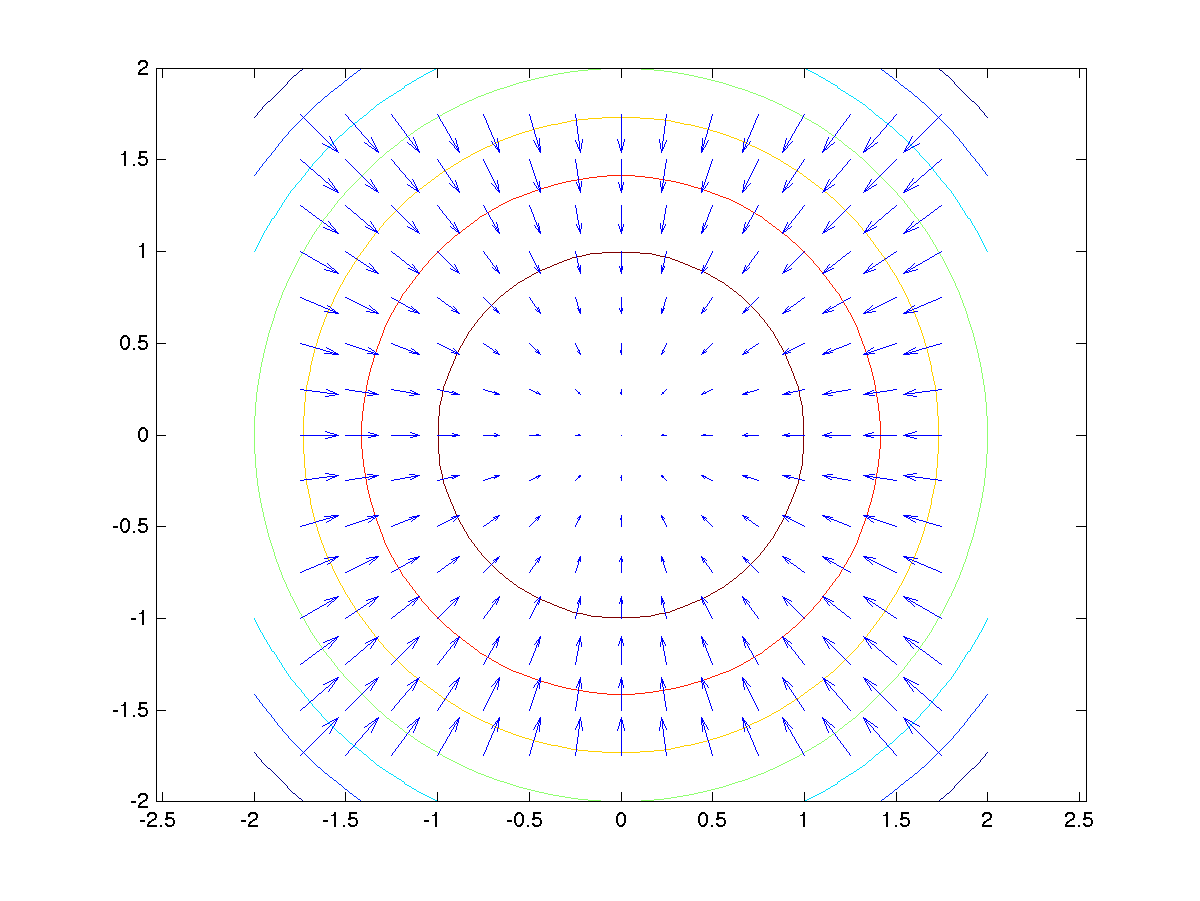
\includegraphics[scale=0.4]{lagrange_1}
    \centering
    \caption {Gradients for level surfaces $f(x,y) = x^{2}+y^{2}$}
    \label{fig:lagrange_1} %\ref{fig:lagrange_1}
\end{figure}

In the context of the solution to the original problem, we will notice that the maximum under constraint occurs when the two surfaces are tangent to each other. This implies that the gradients at the point of maxima are in the same direction (values could be different). We represent this equality using \textbf{Lagrange Multiplier} $\lambda$ (scalar).

\begin{align*}
    \nabla f(x) = \lambda \nabla h(x)
\end{align*}

Thus, now we have $n+1$ equations with us. $n$ equations from the proportionality of the gradients and $1$ from the original constraint. This helps solve for $n$ components of $x$ and the value of $\lambda$. The problem is often formulated as follows

\begin{gather*}
    L(x, \lambda) = f(x) - \lambda (h(x) - c)\\
    \frac{\partial L}{\partial x}(x, \lambda) = 0 \quad \text{and}\quad \frac{\partial L}{\partial \lambda}(x, \lambda) = 0
\end{gather*}

and we can have multiple equality constraints, with a different multiplier for each equation. Using Lagrange multiplier, we converted a constrained optimization problem to an unconstrained one.

\paragraph{Inequality Constraintss} require slightly different handling since we do not have level surfaces anymore. In this context, we have the following problem

\begin{align*}
    \minimize_{x} f(x) \quad f(x):\mathbb{R}^{n} \rightarrow \mathbb{R}\\
    \text{subject to} \quad h(x) = 0 \quad h(x):\mathbb{R}^{n} \rightarrow \mathbb{R}^{m}\\
    \text{and} \quad g(x) \leq 0 \quad h(x):\mathbb{R}^{n} \rightarrow \mathbb{R}^{p}\\
    L(x, \lambda, \mu) = f(x) + \lambda^{T}h(x) + \mu^{T}g(x)
\end{align*}
where $L$ is the Lagrangian and, $\lambda \in \mathbb{R}^{m}$ and $\mu \in \mathbb{R}^{p}$ are thought of as penalties associated with the constraints. This is called the \textbf{Primal}. For a given $\lambda$ and $\mu$ we have an unconstrained problem.\newline

The \textbf{Dual function} is defined as
\begin{align*}
    q(\lambda, \mu) = \min_{x} L(x, \lambda, \mu) \quad q:\mathbb{R}^{m+p} \rightarrow \mathbb{R}
\end{align*}

Notice that the constraint $g(x)$ is violated when $g(x) > 0$. We want to penalize the violation of constraint, meaning, $\mu^{T}g(x) \geq 0$ would make the minimum larger, giving the additional constraint that $\mu \geq 0$.\newline

With the definition of the dual function, the \textbf{Dual problem} is
\begin{gather*}
    \maximize_{\lambda, \mu} q(\lambda, \mu)\\
    \text{with} \quad \mu \geq 0 \quad \text{and} \quad q \text{ is bounded}
\end{gather*}

The idea is to solve the dual problem to get the lower bound on the minimum of the original \textbf{Primal} problem. It is easy to show through the definitions that for the optimal $x^{*}$
\begin{align*}
    q(\lambda, \mu) = \min_{x} L(x, \lambda, \mu) \leq L(x^{*}, \lambda, \mu)\\
    = f(x^{*}) + \lambda^{T}h(x^{*}) + \mu^{T}g(x^{*}) \leq f(x^{*})
\end{align*}

since $x^{*}$ satisfies the original constraints. Thus, the maximum of the dual gives the lower bound on the optimal solution.\newline

In the case of inequalities, we notice the following at the optimal solution
\begin{alignat*}{5}
    &\text{if} \quad g(x^{*}) = 0 \quad &\text{then} \quad &\frac{df}{dx}(x^{*}) +\lambda^{T} \frac{dh}{dx}(x^{*}) + \mu^{T} \frac{dg}{dx}(x^{*}) = 0 &\text{ and } &\mu > 0\\
    &\text{if} \quad g(x^{*}) < 0 \quad &\text{then} \quad &\frac{df}{dx}(x^{*}) +\lambda^{T} \frac{dh}{dx}(x^{*}) + \mu^{T} \frac{dg}{dx}(x^{*}) = 0 &\text{ and } &\mu = 0
\end{alignat*}

where the second case occurs because after assuming $g(x) < 0$, we are just looking at equating the derivatives of $f(x) - \lambda^{T}h(x)$ to zero. The two equations above lead to
\begin{align*}
    g(x^{*}) \leq 0, \quad \mu \geq 0, \quad \mu^{T}g(x^{*}) = 0
\end{align*}
and the last set of conditions are called Karush–Kuhn–Tucker conditions (satisfied only by the optimal point).

\paragraph{Wolfe Dual} is a special case of the above equations. Suppose we do not have any equality constraints, and we also know that $f(x)$ is convex and differentiable, and $g(x)$ is concave (linear will also do) and differentiable. Then the dual is
\begin{align*}
     \max_{\mu} q(\mu) = \max_{\mu} \min_{x} L(x, \mu)
\end{align*}

The minimum occurs at the point where gradient of $L$ is zero and the \textbf{Wolfe Dual} is
\begin{gather*}
    \maximize_{x, \mu} L(x, \mu)\\
    \text{subject to} \quad \mu \geq 0 \quad \text{and} \quad \frac{\partial L}{\partial x}=0
\end{gather*}
along with the KKT conditions valid.

\end{document}